\section{Results}
\label{sec:Results}

In this section, we present the results obtained by running \ApproachName{} and the SBPCG baseline on \CaseStudy{}.
Table~\ref{tab:resultsMeanStDevRQ12} shows the mean values and standard deviations for $Q_{Duration}$ for each \ApproachName{} variant and the SBPCG baseline, while Figure~\ref{fig:results} shows the results in form of boxplots, grouped per host (i.e., the boss of \CaseStudy{}) used in our experiment, (namely Argos, Maia, Orion, Teuthus, and Vermis) and overall (last subfigure with shaded background).  
%The last group of three boxplots, with shaded background, shows the average of all the hosts for each objective function and the baseline. 
Each boxplot is generated from the results of each host obtained from transplantation \ApproachName{} (\simhotep{} and \timhotep{}) or search-based PCG (Base). Each boxplot represents 645 values of a specific host-organ transplantation (\ApproachName{}) or 645 generations from a specific host (Baseline). Each value in the boxplot is the mean value (between the 30 independent runs) of the quality indicator ($Q_{Duration}$) for one of the transplants (\ApproachName{}) or generations (Baseline). 

We can observe that both variants (\simhotep{} and \timhotep{}) obtained better results than the SBPCG baseline (Base). Specifically, \simhotep{} yielded the best results, followed by \timhotep{} and then Base. The variants obtained an average value of 44.85\% in $Q_{Duration}$, with \simhotep{} being the variant that obtained the best results overall (53.31\% in $Q_{Duration}$). \timhotep obtained 36.39\% in the overall $Q_{Duration}$, which also outperformed the baseline. The baseline obtained the worst $Q_{Duration}$. Overall, the results reveal that leveraging simulations as objective function pays off in the context of PCT, yielding 1.5x better results than the \timhotep{} and 2.5x better results than baseline.


\begin{table*}[tb]
\centering
\caption{RQ1-RQ2. Mean values and standard deviations for $Q_{Duration}$ for each approach per Host and Overall.}
\label{tab:resultsMeanStDevRQ12}
\resizebox{.65\textwidth}{!}{
\begin{tabular}{@{}lrrrrrr@{}}
\toprule
    %& \multicolumn{6}{c}{\ApproachName{} with simulation-based variant ($S_{Imhotep}$)}                                           \\ \cmidrule(l){2-7} 
   & Argos            & Maia              & Orion            & Teuthus           & Vermis            & Overall           \\ \midrule
                                   \rowcolor[HTML]{C0C0C0}
\multicolumn{1}{r}{\cellcolor[HTML]{FFFFFF}{$S_{Imhotep}$}} & 43.92 $\pm$ 9.30 & 43.08 $\pm$ 12.09 & 48.86 $\pm$ 8.69 & 60.78 $\pm$ 7.38  & 69.90 $\pm$ 10.52 & 53.31 $\pm$ 14.26 \\ \midrule
    %& \multicolumn{6}{c}{\ApproachName{} with test-based variant ($T_{Imhotep}$)}                                                 \\ \cmidrule(l){2-7} 
    %& Argos            & Maia              & Orion            & Teuthus           & Vermis            & Overall           \\ \midrule
\multicolumn{1}{r}{$T_{Imhotep}$} & 32.17 $\pm$ 6.94 & 29.52 $\pm$ 9.34  & 31.41 $\pm$ 6.83 & 46.33 $\pm$ 10.54 & 42.50 $\pm$ 12.96 & 36.39 $\pm$ 11.72 \\ \midrule
    %& \multicolumn{6}{c}{PCG Baseline (Base)}                                                                             \\ \cmidrule(l){2-7} 
    %& Argos            & Maia              & Orion            & Teuthus           & Vermis            & Overall           \\ \midrule
\multicolumn{1}{r}{Baseline} & 20.15 $\pm$ 1.86 & 8.43 $\pm$ 1.81   & 32.97 $\pm$ 0.85 & 19.53 $\pm$ 1.88  & 25.48 $\pm$ 3.31  & 21.31 $\pm$ 8.32  \\ \bottomrule
\end{tabular}
}
\end{table*}


When analysing whether there is statistical significant differences among the results obtained by \simhotep{} and Base. We found that the obtained $p-values$ for $Q_{Duration}$ are always lower than $4.01x10^{-23}$  (see Table \ref{tab:resultsWilcEffRQ1}). This is below the significance threshold value, so we can comfortably state that \simhotep{} provides significant better values for $Q_{Duration}$ with respect to Base. We also observe that all the  A12 effect size values are large (see Table \ref{tab:resultsWilcEffRQ1}), thus confirming the practical magnitude of such a difference. Thus, we conclude that:

\noindent \textbf{Answer to RQ$_1$} \simhotep{} performance far surpasses the baseline with statistically significant results and large effect size in all cases, and exhibiting a remarkable overall enhancement of 250\%.


\begin{table}[tb]
	\centering
	\caption{RQ1. Mann-Withney U pair-wise test results / Vargha-Delaney Â$_{12}$ effect sizes obtained comparing \simhotep{} Vs. Base per host and overall. Â$_{12}$: Large -- L.}
	\label{tab:resultsWilcEffRQ1}
	\resizebox{.4\columnwidth}{!}{
	\begin{tabular}{@{}lr@{}}
		\toprule
		Boss    & $p-Value$ / Â$_{12}$           \\ \midrule 
		Argos   & $3.25x10^{-23}$  / 0.99 (L)    \\
		Maia    & $3.25x10^{-23}$  /  1.0 (L)    \\
		Orion   & $4.01x10^{-23}$  / 0.98 (L)    \\
		Teuthus & $3.25x10^{-23}$  /  1.0 (L)    \\
		Vermis  & $3.25x10^{-23}$  /  1.0 (L)    \\
		Overall & $1.41x10^{-107}$ / 0.98 (L)    \\
		\bottomrule
	\end{tabular}
}
\end{table}

\begin{table}[tb]
    \centering
    \caption{RQ2. Mann-Withney U pair-wise test results / Vargha-Delaney Â$_{12}$ effect sizes obtained comparing \simhotep{} Vs. \timhotep{} per host and overall. Â$_{12}$: Large -- L.}
	\label{tab:resultsWilcEffRQ2}
	\resizebox{.4\columnwidth}{!}{
    \begin{tabular}{@{}lr@{}}
    \toprule
    Boss    & $p-Value$ / Â$_{12}$           \\ \midrule 
    Argos   & $1.28x10^{-18}$ / 0.85 (L)     \\
    Maia    & $6.64x10^{-18}$ / 0.85 (L)     \\
    Orion   & $4.95x10^{-22}$ / 0.95 (L)     \\
    Teuthus & $3.60x10^{-18}$ / 0.87 (L)     \\
    Vermis  & $8.86x10^{-23}$ / 0.95 (L)     \\
    Overall & $6.58x10^{-93}$ / 0.82 (L)     \\
    \bottomrule
    \end{tabular}
}
    \end{table}
    
As for the comparison between \simhotep{} and \timhotep{} (RQ2),  we observe that all the $p-values$ achieved when comparing the $Q_{Duration}$ distributions provided by the two \ApproachName{} variants are smaller than the significance threshold, thus indicating that the difference in solution quality is statistically significant in favour of \simhotep{}, and always with a large A12 effect size (see Table \ref{tab:resultsWilcEffRQ2}). Therefore, we conclude that:

\noindent  \textbf{Answer to RQ$_2$} \simhotep{} provides significantly better results than \timhotep{} in the context of automated content generation through transplantation, with a large effect size in all cases examined. The efficacy of \simhotep{} demonstrates a 150\% enhancement overall compared to the outcomes of \timhotep{}.

\begin{figure*}[tb]
    \centering
    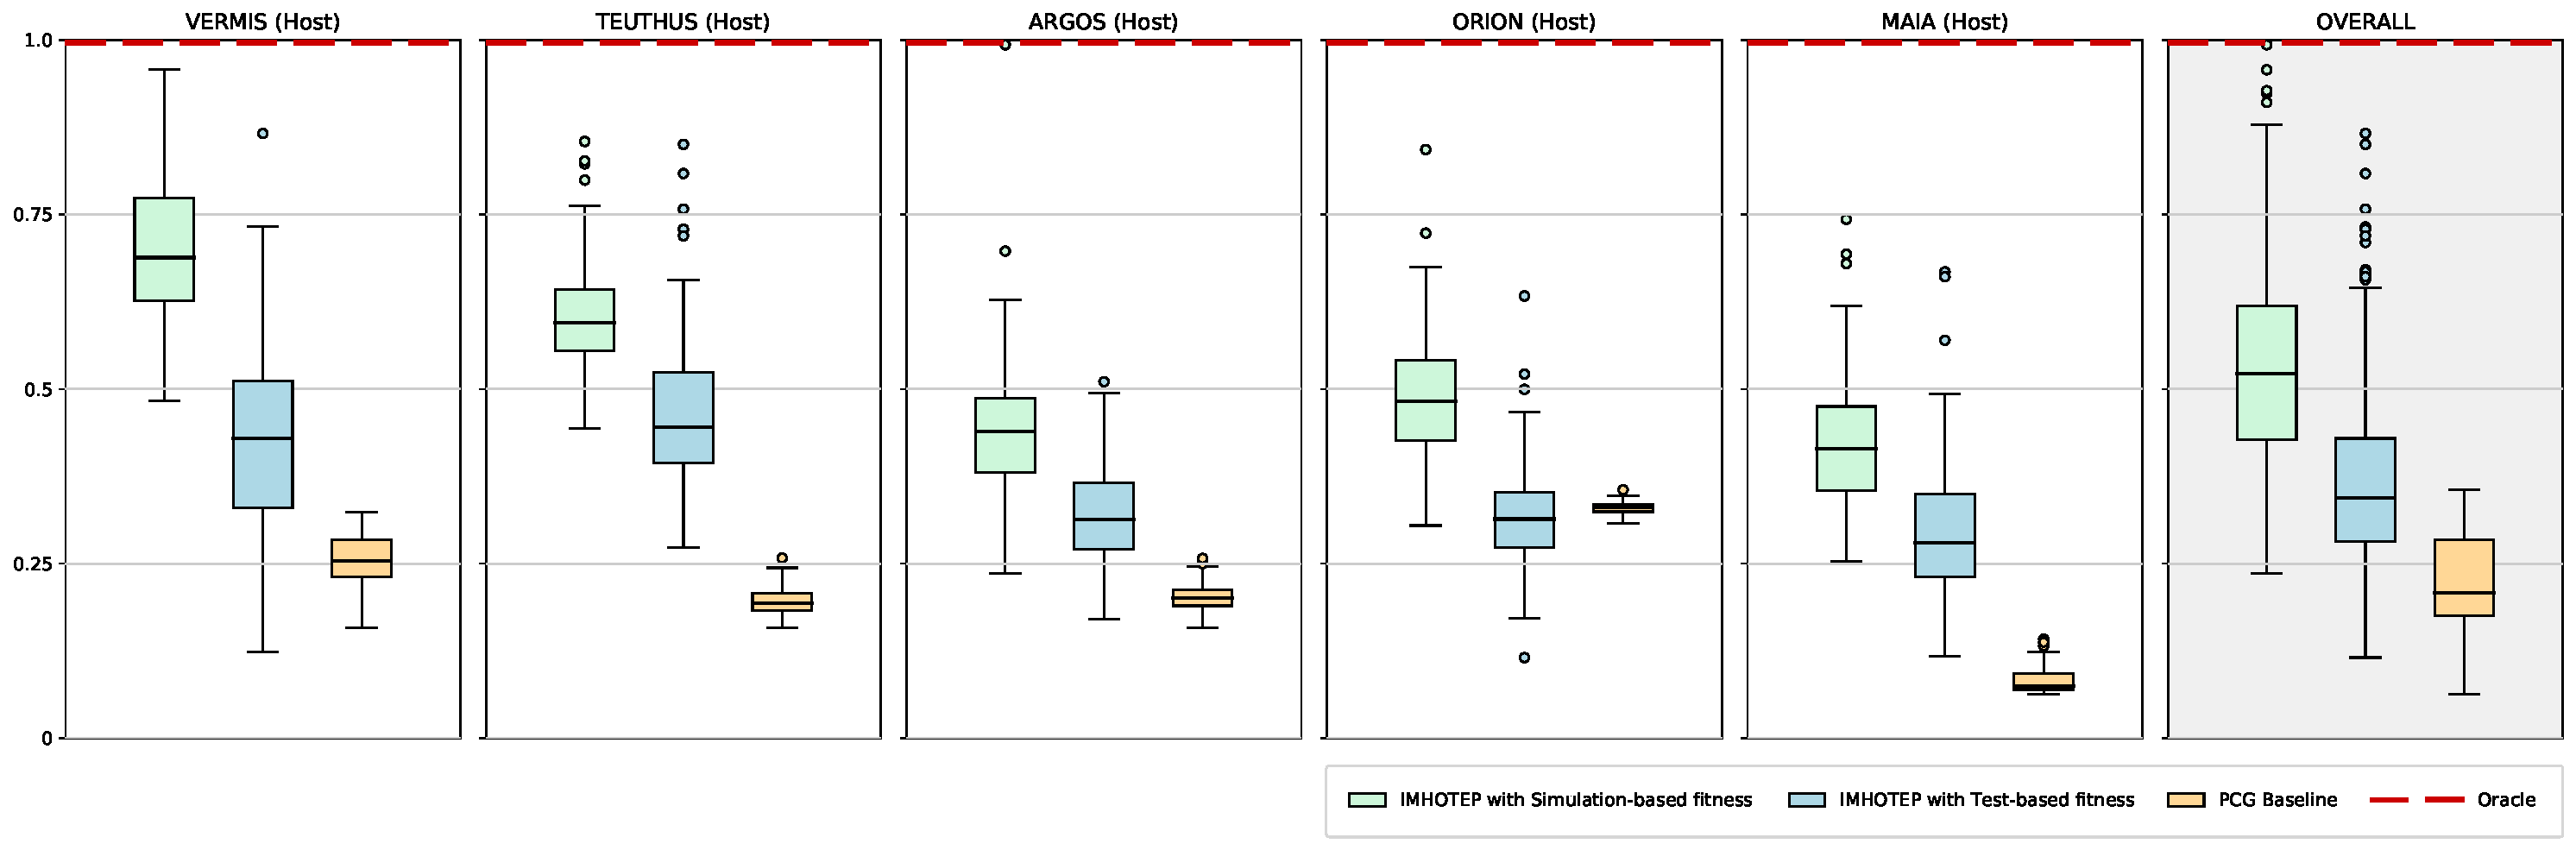
\includegraphics[width=0.8\textwidth]{Figures/Imhotep_with_legend_and_oracle_average-v4.pdf}
    \caption{RQ1-RQ2. Results of our \ApproachName{} (simulation-based and test-based) and the SBPCT baseline for the quality measurement ($Q_{Duration}$) for each of the \CaseStudy{} Host and Overall.}
    \label{fig:results}
\end{figure*}